\documentclass[a4paper,titlepage,12pt]{report}
\usepackage[brazil]{babel}
\usepackage[latin1]{inputenc}
\usepackage{epsfig}
\usepackage{times}
\usepackage{amsfonts,amssymb,latexsym,eucal,amsmath,theorem,amscd}
\usepackage{graphicx}
\usepackage[T1]{fontenc}

\usepackage{color}
\usepackage{longtable}
\usepackage{fancyhdr}
\usepackage{fancyvrb}
\usepackage{verbatim}

\usepackage{graphicx,url}
\usepackage{amssymb}
\usepackage{epsfig}

\usepackage[portuguese]{nomencl}

\setlength{\textheight}{247mm}
\setlength{\textwidth}{155mm}
\setlength{\topmargin}{-0.4mm}
\setlength{\oddsidemargin}{5.4mm}
\setlength{\voffset}{-13mm}
\usepackage{colortbl}

\sloppy
% Comandos de estilo e espacamento ----------------------------------------
\newlength{\defbaselineskip}
\setlength{\defbaselineskip}{\baselineskip}
\newcommand{\setlinespacing}[1]%
           {\setlength{\baselineskip}{#1 \defbaselineskip}}

\newcommand{\emptypage}
           {\newpage\thispagestyle{empty}\mbox{}}

\setcounter{topnumber}{2}
\renewcommand{\topfraction}{.7}
\setcounter{bottomnumber}{1}
\renewcommand{\bottomfraction}{.3}
\setcounter{totalnumber}{3}
\renewcommand{\textfraction}{.2}
\renewcommand{\floatpagefraction}{.5}
\setcounter{dbltopnumber}{2}
\renewcommand{\dbltopfraction}{.7}
\renewcommand{\dblfloatpagefraction}{.5}
\renewcommand{\appendixname}{Anexo}

\oddsidemargin -28pt
\evensidemargin -28pt
\marginparwidth 50pt
\marginparsep 5pt
\topmargin -27pt
\hoffset 15mm
\textheight 237mm
\textwidth 155mm
\renewcommand{\baselinestretch}{1.5}
% ------------------------------------------------------------------------

\renewcommand{\nomname}{Lista de Siglas e Abreviaturas}

\makenomenclature

\begin{document}

\pagestyle{empty}

\begin{center}
{\textbf{\Large \textsc{Universidade Federal de Campina Grande}}}
\end{center}

\begin{center}
\textbf{{\Large \textsc{Centro de Engenharia El�trica e
Inform�tica}}}
\end{center}

\begin{center}
\textbf{{\Large \textsc{Unidade Acad�mica de Sistemas e
Computa��o}}}
\end{center}

\begin{center}
{\large \textsc{\textbf{Gradua��o em Ci�ncia da Computa��o}}}
\end{center}


~\\


\begin{center}
\textsc{Relat�rio de Est�gio}\\
{\Large \textsc{\textbf{An�lise Comparativa do Uso de Tecnologias de Grades Computacionais de Desktop}}}
\end{center}
~\\

\begin{center}
\large{\textsc{Ricardo Ara�jo Santos}}\\
\textsc{Estagi�rio}\\
\end{center}
~
% \begin{quote}
% \small{Monografia submetida � Coordena��o do Curso de Ci�ncia da
% Computa��o da Universidade Federal de Campina Grande - Campus I como
% resultado da disciplina Est�gio Integrado.}
% \end{quote}
% ~\\
% 
% \begin{center}
% \textsc{�rea de Concentra��o: Ci�ncia da Computa��o }\\
% \textsc{Linha de Pesquisa: Sistemas Distribu�dos - Sistemas Peer-to-Peer - Grades Computacionais}\\
% \end{center}
% ~\\

\begin{center}
\textsc{Raquel Vigolvino Lopes}\\
\textsc{Orientadora Acad�mica}\\
\end{center}
~

\begin{center}
\textsc{Marcus Williams Aquino de Carvalho}\\
\textsc{Supervisor T�cnico}\\
\end{center}
~

\begin{center}
{\small \textsc{Campina Grande, Para�ba, Brasil}}\\
{\small \textsc{$\copyright$ Ricardo A. Santos, Julho de 2009}}
\end{center}

\newpage
\cleardoublepage
\newpage

% Configura os n�meros das p�ginas para algarismos romanos
\pagestyle{plain}
\pagenumbering{roman}

% -------- Lista de Figuras --------- %

%\listoffigures
%\newpage

% ------------- �ndice -------------- %



\clearpage
%% Corpo do documento -------------------
%
% Configura os n�meros das p�ginas para algarismos indo-arabicos
\pagestyle{plain}
\setcounter{page}{1}
\pagenumbering{arabic}

\newenvironment{worduglystyle}[1]
{\spaceskip=.33em plus \hsize #1}
{}

%%%%%%%%%%%%%%%%%%%%%%%%%%%%%%%%%%%%%%%%%%%%%%%%%%%%%%%%%%%%%%%%%%%%%%%%%%%%%%%%%
%%% Definicao do cabecalho: secao do lado esquerdo e numero da pagina do lado direito
\pagestyle{fancy}
\addtolength{\headwidth}{\marginparsep}\addtolength{\headwidth}{\marginparwidth}\headwidth
= \textwidth
%\renewcommand{\sectionmark}[1]{\markboth{#1}{}}
\renewcommand{\sectionmark}[1]{\markright{\thesection\ #1}}\lhead[\fancyplain{}{\bfseries\thepage}]%
         {\fancyplain{}{\emph{\rightmark}}}\rhead[\fancyplain{}{\bfseries\leftmark}]%
             {\fancyplain{}{\bfseries\thepage}}\cfoot{}

%%%%%%%%%%%%%%%%%%%%%%%%%%%%%%%%%%%%%%%%%%%%%%%%%%%%%%%%%%%%%%%%%%%%%%%%%

\begin{center}
{\textsc{\textbf{An�lise Comparativa do Uso de Tecnologias de Grades Computacionais de Desktop}}}
\end{center}

Aprovado em \rule{3cm}{0.1mm}\\

\begin{center}
{\textsc{\textbf{Banca Examinadora}}}\\
\end{center}

\begin{center}
	\vspace{2cm}
	\rule{12cm}{0.1mm}\\
	\textbf{Prof$^{a}$. Dr$^{a}$. Raquel Vigolvino Lopes}\\
	ORIENTADORA ACAD�MICA

	\vspace{3cm}
	\rule{12cm}{0.1mm}\\
	\textbf{Prof. Dr. Francisco Vilar Brasileiro}\\
	MEMBRO DA BANCA\\

	\vspace{3cm}
	\rule{12cm}{0.1mm}\\
	\textbf{Prof$^{a}$. Dr$^{a}$. Joseana Mac�do Fechine}\\
	MEMBRO DA BANCA\\

\end{center}





\chapter*{Agradecimentos}
\label{agradecimentos}

Ao Laborat�rio de Sistemas Distribu�dos pela oportunidade de realizar o est�gio. Aos supervisores pela orienta��o. Aos integrantes do LSD pelas dicas e � equipe de suporte pela paci�ncia.


\chapter*{Apresenta��o}
\label{apresentacao}

Como parte das exig�ncias do curso de Ci�ncia da Computa��o, da Universidade Federal de Campina Grande, para cumprimento da disciplina de est�gio integrado, � apresentado o relat�rio de est�gio seguinte.

O est�gio foi realizado no LSD\nomenclature{LSD}{Laborat�rio de Sistemas Distribu�dos} sob supervis�o acad�mica da professora doutora Raquel Vigolvino Lopes e t�cnica de Marcus Williams Aquino de Carvalho, no per�odo 2009.1.

O conte�do do relat�rio est� distribu�do conforme descri��o a seguir:

\begin{description}
  \item[Se��o 1 - ] Introdu��o 
  \item[Se��o 2 - ] Objetivos
  \item[Se��o 2 - ] Ambiente de Est�gio 
  \item[Se��o 3 - ] Fundamenta��o Te�rica e Tecnologias Utilizadas 
  \item[Se��o 4 - ] Metodologia 
  \item[Se��o 4 - ] Resultados Obtidos 
  \item[Se��o 5 - ] Considera��es Finais 
  \item[] Refer�ncias Bibliogr�ficas 
\end{description}


\abstract{O uso de grades computacionais de desktop no contexto da pesquisa cient�fica � uma alternativa barata a aquisi��o de supercomputadores ou clusters dedicados e muito tem sido pesquisado nessa �rea. Algumas tecnologias de grades computacionais t�m se tornado bem conhecidas e aplicam na pr�tica muito do conhecimento produzido nas pesquisas. Este est�gio tem por objetivo comparar e contrastar algumas dessas tecnologias identificando caracter�sticas predominantes nos pacotes de \textit{middleware} mais em uso atualmente.}


\tableofcontents

\printnomenclature[1cm]

\listoffigures

\listoftables

\chapter{Introdu��o}
\label{introducao}

A pesquisa cient�fica em algumas �reas tem demandado cada vez mais poder computacional, seja para a realiza��o de simula��es como para a execu��o de experimentos. Uma sa�da na\-tu\-ral � a aquisi��o de supercomputadores ou m�quinas dedicadas (\textit{clusters}) exclusivamente � computa��o paralela, o que nem sempre � poss�vel dado seu elevado custo. As grades computacionais \cite{berman, kesselman} surgiram com a id�ia de resolver tais problemas computacionais de maneira eficiente e com baixo custo, atrav�s do compartilhamento de recursos.

Uma forma comum de compartilhamento de recursos faz uso de poder computacional ocioso, formando o que se chama no contexto desse trabalho de grades computacionais de \textit{desktop}. Exemplos de grades desse tipo s�o: Condor~\cite{condor:history}, BOINC~\cite{boinc}, XtremWeb~\cite{xtremweb} e OurGrid~\cite{ourgrid}.

Muito tem sido publicado em confer�ncias e jornais sobre essas ferramentas. No entanto, n�o s�o conhecidos estudos emp�ricos que visem uma caracteriza��o do uso das ferramentas disponibilizadas, impossibilitando identificar o estado-da-pr�tica desta �rea. Acredita-se que um estudo pr�tico, em contrapartida aos estudos te�ricos conhecidos, � de grande import�ncia tanto para identifica��o de lacunas quanto para sele��o do melhor servi�o em diferentes contextos.

%       - import�ncia do est�gio para a forma��o profissional;
Realizar esse tipo de pesquisa num est�gio � uma oportunidade de p�r em pr�tica alguns conhecimentos adquiridos durante a vida acad�mica do estudante de gradua��o j� que � feita a ponte entre as teorias aprendidas nas disciplinas e como elas s�o usadas na pr�tica por um pesquisador.

%       - delimita��o do est�gio realizado, no tempo e espa�o, ou seja, informar pontualmente onde o est�gio foi realizado e o per�odo utilizado;
O est�gio do qual se trata esse relat�rio foi realizado como disciplina do curr�culo optativo do Curso de Bacharelado em Ci�ncia da Computa��o no per�odo 2009.1 e realizado no Laborat�rio de Sistemas Distribu�dos na Universidade Federal de Campina Grande.

\section{Objetivos}
\label{objetivos}

O principal objetivo desse trabalho � comparar de forma qualitativa o uso das principais tecnologias de grades desktops ou oportunistas da atualidade.

Como objetivos espec�ficos espera-se:

\begin{itemize}
  \item Realizar um levantamento bibliogr�fico sobre as grades desktop ou oportunistas mais usadas atualmente;
  \item Levantar m�tricas que possam ser usadas nesse estudo comparativo qualitativo;
  \item Comparar qualitativamente, com base nas m�tricas definidas, as grades identificadas no in�cio do est�gio. 
\end{itemize}


\chapter{Ambiente de Est�gio}
\label{ambiente}

O est�gio foi desenvolvido no Laborat�rio de Sistemas Distribu�dos (LSD) do Departamento de Sistemas e Computa��o (DSC) da Universidade Federal de Campina Grande.

O laborat�rio foi criado em 1996, como forma de aglutinar pesquisadores e alunos do DSC e de outros departamentos em torno de projetos na �rea de Sistemas Distribu�dos. A\-tu\-al\-men\-te o LSD � coordenado pelo professor Francisco Brasileiro. As pesquisas do LSD est�o concentradas em Grades Computacionais, Sistemas \textit{Peer-to-Peer}, \textit{Cloud Computing}, Toler�ncia a Falhas, Desenvolvimento de Software Distribu�do e Aplica��es Industriais.

\section{Estrutura F�sica}
\label{estrutura}

O LSD est� instalado num pr�dio com $550m^2$ de �rea e conta com a colabora��o de dezenas de alunos desenvolvendo trabalhos de doutorado, mestrado e inicia��o cient�fica, al�m de v�rios pesquisadores. Os diferentes projetos em execu��o est�o distribu�dos em 8 (oito) salas climatizadas, cada uma contanto com quadro branco, pinc�is e um acervo bibliogr�fico de diversos temas em computa��o e engenharia. Cada pessoa possui um posto de trabalho individual, com m�quinas conectadas � Internet via POP-PB da RNP\nomenclature{RNP}{Rede Nacional de Pesquisa}.

\vspace{1cm}
\noindent
\textbf{Endere�o}: Universidade Federal de Campina Grande\newline
Departamento de Sistemas e Computa��o\newline
Laborat�rio de Sistemas Distribu�dos\newline
Av. Apr��gio Veloso, 882 - Bloco CO\newline
Bodocong�, CEP 58109-970 Campina Grande - PB, Brasil\newline
Fone: +55 83 3310 1365\newline
Fax: +55 83 3310 1498

\section{Rucursos Utilizados}

\subsection{Hardware}

Foram disponibilizados quatro computadores de configura��es distintas. 

\subsection{Software}

Os recursos de software utilizados foram os seguintes:

\begin{itemize}
  \item Eclipse: Como ambiente de desenvolvimento da aplica��o Java usada para testar as grades computacionais. Al�m disso, o Eclipse em conjunto com o plugin Texlipse foi usado como editor de texto \LaTeX;
  \item VServer: Como ambiente de m�quinas virtuais.
\end{itemize}


\chapter{Fundamenta��o Te�rica}
\label{fundamentacao}

Esta se��o tem por finalidade introduzir alguns dos conceitos abordados no est�gio. Primeiro � dada uma contextualiza��o com o hist�rico das grades computacionais. Depois, s�o definidos alguns conceitos importantes e dados exemplos de algumas aplica��es executadas em grades computacionais.    

\section{Grades Computacionais}

\subsection{Hist�rico}

Usar computadores ociosos conectados em rede para execu��o de tarefas n�o � uma id�ia nova. Em 1982, o \textit{Worm} da Xerox executava nos \textit{desktops} da empresa~\cite{xerox:worm} aplica��es que variavam muito de objetivo. Os \textit{worms} se espalhavam na rede detectando m�quinas ociosas e se replicando, e realizavam tarefas complexas como diagn�stico de problemas na Ethernet e at� a cria��o de anima��es em tempo real.

No in�cio dos anos 90, com a difus�o dos \textit{applets} Java~\cite{java}, surgiram sistemas como Javelin~\cite{java:javelin} e Bayanihan~\cite{java:bayanihan}. Tais aplica��es se propagavam atrav�s dos navegadores, o que era uma vantagem dado que o tr�fego era realizado via \textit{Hypertext Transfer Protocol} (HTTP\nomenclature{HTTP}{Hypertext Transfer Protocol}). Os sistemas eram flex�veis e facilmente instal�veis. No entanto, os navegadores executavam os \textit{applets} em \textit{sandboxes} o que tornava imposs�vel o acesso a alguns servi�os como monitores de carga de CPU e mem�ria principal. As aplica��es executadas eram res\-tri\-tas tamb�m j� que n�o podiam realizar leitura ou escrita no sistema de arquivos local. A escalabilidade n�o foi provada dado que esses sistemas n�o foram implantados em mais que algumas dezenas de recursos. Al�m disso, n�o existiam ferramentas de ger�ncia para tais aplicativos.

Ainda nos anos 90, Anderson, Culler e Patterson~\cite{now} argumentavam que as \textit{Networks of Workstations} (NOWs)\nomenclature{NOW}{Network of Workstations} podiam ter um desempenho igual ou maior que m�quinas com Massively Parallel Processor (MPP)\nomenclature{MPP}{Massively Parallel Processor}. Este argumento era suportado por tr�s particularidades: (i) a capacidade das redes locais (Local-area Networks - LANs)\nomenclature{LAN}{Local-area Network} permitia a escala das aplica��es com protocolos ass�ncronos de transfer�ncia de dados; (ii) as m�quinas \textit{desktop} estavam me\-lho\-ran\-do significativamente em poder de processamento; e (iii) opera��es de I/O \nomenclature{I/O}{Input/Output} continuavam a ser um gargalo para supercomputadores e que podia ser contornado com a paraleliza��o nas NOWs.

Foi tamb�m nos anos 90, que um sistema chamado Condor~\cite{condor:history} foi ganhando espa�o. O Condor � um \textit{middleware} para execu��o distribu�da de aplica��es em \textit{batch}. O Condor originalmente foi concebido para uso em ambientes LAN, mas atualmente permite a comunica��o em escala global, chegando a ter cerca de 274498 m�quinas em 1897 \textit{pools} em Mar�o de 2009\cite{condor:status}.

A difus�o da Internet no fim dos anos 90 trouxe a possibilidade de conectar milh�es de \textit{desktops} ao redor do mundo e com isso projetos de computa��o volunt�ria como, por exemplo, o SETI@home~\cite{seti}, ganharam popularidade. A computa��o volunt�ria fazia uso dos \textit{desktops} de pessoas comuns ao redor do mundo para a execu��o de aplica��es altamente paraleliz�veis em troca de prest�gio social. O SETI@home, por exemplo, divulga os maiores contribuintes na sua p�gina inicial al�m de fornecer prote��es de tela com imagens em tr�s dimens�es relacionadas � pesquisa.

Ap�s isso, v�rios projetos em universidade come�aram a desenvolver sistemas para aplica��es em grades de \textit{desktop}, entre eles o XtremWeb~\cite{xtremweb} e BOINC~\cite{boinc}. Algumas empresas tamb�m decidiram lan�ar seus produtos destinados a comunidade corporativa como o Entropia~\cite{entropia}, United Devices (apud \cite{uniteddevices}). E mais recentemente, em 2004, InteGrade~\cite{integrade} e OurGrid~\cite{ourgrid} surgem como iniciativas nacionais no uso de poder computacional de \textit{desktops} ociosos.

\subsection{Conceitos}

Grades computacionais s�o sistemas distribu�dos caracterizados pelo compartilhamento de recursos heterog�neos localizados em diferentes dom�nios administrativos (federados)~\cite{thegrid2}. O \textit{middleware} de grade computacional � a camada de software que possibilita a comunica��o entre os recursos da grade e as aplica��es de forma consistente e homog�nea. A arquitetura do middleware define o prop�sito, as fun��es e intera��es entre os componentes para gerenciar recursos tais como processamento e armazenamento~\cite{middleware}.

N�o existe um consenso na literatura sobre a classifica��o das grades computacionais. Por�m alguns conceitos se destacam e s�o necess�rios para o entendimento desse trabalho.

%O que �?
As grades computacionais s�o chamadas oportunistas quando os recursos que comp�em a grade s�o usados quando est�o ociosos. Estudos mostram que esta��es de trabalho ficam ociosas entre 60\% e 80\% do seu tempo de vida\cite{oportunistic}. Dessa forma, grades oportunistas oferecem uma forma barata de se prover computa��o de alta vaz�o usando esta��es \textit{desktop} ociosas. 

Nesse contexto existem tamb�m as grades de \textit{desktops}, que podem ser definidas como um conjunto de \textit{desktops} conectados em rede com a inten��o de se prover computa��o distribu�da de alta vaz�o. Os recursos de processamento e armazenamento s�o utilizados de forma oportunista, logo s�o, naturalmente, grades oportunistas, ou seja, as aplica��es do dono da m�quina t�m prioridade sobre as aplica��es executadas na grade e estas s�o executadas somente quando n�o h� demanda do dono da m�quina. Al�m disso, a disponibilidade do recurso depende de fatores, como falha de rede, \textit{hardware} ou \textit{software}, e n�o existe nenhuma garantia sobre os recursos doados aos clientes da grade. Al�m da volatilidade dos recursos, outra caracter�stica que se destaca � a heterogeneidade dos recursos que comp�em a grade no tocante a processadores, sistema operacional, freq��ncia de \textit{clock}, espa�o em disco e velocidade de acesso � rede, por exemplo.

Quando usu�rios dom�sticos passam a doar recursos ociosos para a grade sem, em troca, consumir recursos da grade, tem-se o que se chama de computa��o volunt�ria. O dom�nio sobre os recursos da grade estende as fronteiras dos laborat�rios envolvidos e a comunidade passa a ter certo envolvimento com a pesquisa. Isso acontece, por exemplo, com o projeto SETI@Home onde qualquer pessoa pode doar recursos para a grade e em troca os doadores mais ativos s�o listados na p�gina principal do projeto.

Em contrapartida, existem ainda as grades computacionais de servi�o. Nesse caso, organiza��es virtuais tipicamente mant�m uma grade formada por recursos dedicados e oferecem garantias de Qualidade de Servi�o (\textit{Quality of service} - QoS\nomenclature{QoS}{Quality of Service}) a seus clientes. Al�m disso, os recursos s�o fechados por pol�ticas de acesso restrito firmados por essas organiza��es vir\-tuais. Este trabalho mant�m o foco nas grades computacionais de \textit{desktop} classificadas como oportunistas. 

Al�m dos termos apresentados, as pr�ximas se��es usam alguns termos informalmente convencionados pela comunidade cient�fica. Cliente � aquele que deseja executar aplica��es ou \textit{jobs}, que s�o conjuntos de tarefas ou \textit{tasks}. O cliente submete aplica��es para a grade de modo que o escalonador do servidor envie tarefas para \textit{workers} que estejam dispon�veis. Os \textit{workers}, por sua vez, s�o \textit{daemons} que executam nas m�quinas (recursos) doadas � grade.

Uma vez definidos os termos usados, pode-se pensar em caracter�sticas de um modelo ideal de grade de \textit{desktops}. Algumas s�o:

\begin{enumerate}
  \item Escalabilidade: A vaz�o do sistema deve aumentar com a adi��o de m�quinas no sistema;
  \item Toler�ncia a faltas: O sistema deve tolerar falhas tanto do servidor de aplica��es como dos \textit{workers}. Nesse trabalho, incluem-se no termo falhas n�o s� as falhas de \textit{hardware} e \textit{software} como tamb�m, a interrup��o da execu��o do \textit{worker} por atividade do teclado ou mouse, ou ainda, por desligamento da m�quina, por exemplo;
  \item Prote��o: A m�quina deve ser protegida de aplica��es maliciosas que sejam submetidas � grade;
  \item Gerenciabilidade: Com o grande n�mero de recursos sendo doados na grade em diversos sites diferentes, torna-se necess�rio que atividades gerenciais como instala��o, atualiza��o e monitoramento possam ser efetivadas automaticamente;
  \item N�o-intrusividade: O usu�rio dono da m�quina deve ter prioridade sobre as aplica��es que queiram executar na grade. A aplica��o pode ser finalizada e recome�ada em outra m�quina ou pode ser pausada e recome�ada assim que o dono da m�quina n�o a estiver utilizando.
  \item Usabilidade: O usu�rio n�o deve encontrar obst�culos para executar uma aplica��o na grade, de modo que n�o seja necess�rio modificar aplica��es. Isso impediria a execu��o de aplica��es legadas ou de c�digo propriet�rio ao qual o usu�rio n�o tem acesso para fazer as modifica��es necess�rias para executar na grade.
\end{enumerate}

No contexto deste trabalho, dois desses aspectos foram analisados: gerenciabilidade e usabilidade.
 
\subsection{Arquitetura}
\label{arquitetura}

Cada middleware de grades de desktops define uma arquitetura formada por componentes que desempenham diferentes pap�is na grade e cada um estabeleceu sua forma pr�pria de nomear tais componentes, mas em geral eles desempenham servi�os bem semelhantes em tr�s n�veis distintos definidos em~\cite{uniteddevices} (ver Figura~\ref{figure:modelo}): 

\begin{enumerate}
  \item O cliente: o cliente possui o c�digo execut�vel da aplica��o, que ser� submetida para execu��o na grade. Assim, o m�dulo cliente � usado para controlar a execu��o das tarefas, servindo de \textit{front-end} entre a grade e seus usu�rios;
  \item A ger�ncia de aplica��o e recursos: armazena informa��es sobre as aplica��es at� que recursos estejam dispon�veis para execut�-la e realiza o casamento entre aplica��es e recursos dispon�veis;
  \item Os \textit{workers}: s�o os recursos da grade, nos quais as tarefas do cliente executam de fato.
\end{enumerate}

\begin{figure}[htp]
\begin{center}
  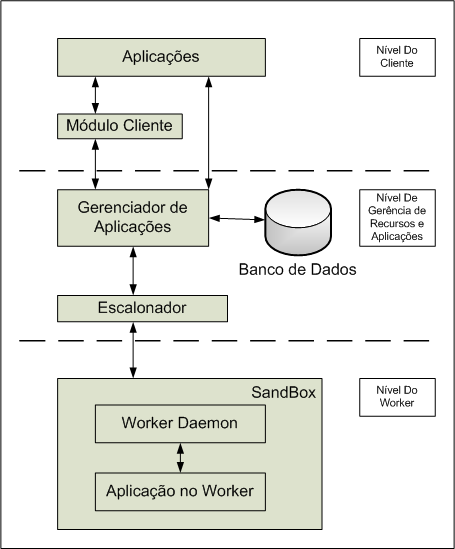
\includegraphics[width=10cm]{figures/modelo.png}
  \caption[Modelo Geral de Grades Computacionais de Desktop]{Modelo Geral de Grades Computacionais de Desktop}
  \label{figure:modelo}
\end{center}
\end{figure}

\subsection{Aplica��es}

V�rios tipos de aplica��es podem tirar proveito da execu��o em grades de \textit{desktops}. Entre as �reas mais comuns se encontram a biologia computacional~\cite{biology:athome,biology:fightaids}, os modelos clim�ticos~\cite{climate} e aplica��es de f�sica~\cite{physics}. Com o advento da computa��o em grades de \textit{desktop}, foi poss�vel levar as simula��es e experimentos cient�ficos a um novo patamar, dada a possibilidade de explorar grandes faixas de par�metros nos simuladores ou mesmo realizar simula��es e experimentos mais complexos.

Qualquer aplica��o distribu�da pode ser executada numa grade computacional. Aplica��es paralelas especialmente s�o as que mais podem tirar proveito desse tipo de arquitetura distribu�da.  
Uma classe de aplica��es paralelas not�vel � a das aplica��es \textit{Bag-of-Tasks} (BoT)\nomenclature{BoT}{Bag-of-Tasks} que s�o aquelas aplica��es paralelas cujas tarefas s�o independentes entre si, ou seja, n�o h� comunica��o entre as tarefas. Essas aplica��es s�o bastante comuns na pr�tica, presentes em minera��o de dados, varredura de par�metros, simula��es e c�lculo de fractais, por exemplo~\cite{labs}.


\chapter{Metodologia}
\label{metodologia}

A id�ia deste trabalho � realizar uma an�lise comparativa a respeito do uso das grades computacionais de desktop mais populares da atualidade. Optou-se por uma abordagem qualitativa para avaliar o uso de cada ferramenta. Inicialmente foi constru�da uma base de informa��es sobre as ferramentas estudadas, tais como artigos e documenta��o das ferramentas. Em um segundo momento, foram escolhidas algumas m�tricas a serem usadas como base para a compara��o entre estas ferramentas. � luz de tais m�tricas, as ferramentas foram utilizadas e foi realizada uma an�lise comparativa das ferramentas que refletem o estado da pr�tica nesta �rea. As m�tricas levaram em conta as diversas fases do uso das tecnologias como a instala��o e o uso da grade em si, como tamb�m custos de manuten��o e prepara��o de aplica��es para execu��o na grade, por exemplo.

Dessa forma, pode se dizer que a metodologia deste trabalho se divide nas seguintes etapas:

\begin{itemize}
  \item Formula��o do problema e dos procedimentos da pesquisa:
\begin{itemize}
  \item Defini��o do problema;
  \item Identifica��o das ferramentas a serem analisadas;
\end{itemize}
  \item Planejamento das m�tricas avaliadas:
\begin{itemize}
  \item Determinar o que deve ser estudado nas ferramentas;
  \item Identificar aspectos comuns nas ferramentas; 
\end{itemize}
  \item Determina��o os cen�rios de experimenta��o:
\begin{itemize}
  \item Determinar a sele��o de amostras;
  \item Verificar e validar a sele��o de amostras no tocante a representar a popula��o; 
\end{itemize}
  \item Realiza��o os experimentos e coleta de dados;
  \item Desenvolvimento de um plano de an�lise da amostra:
\begin{itemize}
  \item Filtrar dados relevantes;
\end{itemize}
  \item Processar e analisar os dados obtidos gerando uma tabela comparativa das ferramentas usadas.
\end{itemize}

% Metodologia Cient�fica
% 
% M�todos Qualitativos
%     Se ocupam de vari�veis que n�o podem ser medidas, apenas observadas.
% 
%     * Pesquisa observacional: observar o ambiente mas n�o modific�-lo
%           o perspectiva filos�fica:
%                 + positivistas: existem vari�veis objetivas. Tenta falar em teorias, provar ou desprov�-las.
%                       # Descritiva: Descreve de forma objetiva e direta eventos e fatos de interesse.
%                       # Explorat�ria: prop�e novas teorias, observa��es e m�tricas.
%                 + interpretativistas: n�o existem vari�veis objetivas. Tudo depende da interpreta��o do observador.
%                 + cr�tica: entende o mundo como uma constru��o hist�rica e social de rela��es de poder e domina��o. Vai atr�s dessas rela��es.
%           o Estilo:
%                 + Estudo de Caso: intera��o do pesquisador com o sujeito � semi-formal.
%                 + Etnografia: o pesquisador vive e trabalha com o sujeito.
%           o T�cnicas: o problema � o rigor. Garantir confiabilidade, validade (controlar a subjetividade ou vi�s do pesquisador) e generabilidade
%                 + amostragem fundamentada em teoria ou direcionada (purposive or theoretical sampling): sele��o das amostras n�o � aleat�ria, busca casos extremos
%                 + separa��o de observa��o e teoriza��o: coleta de dados e teoriza��o independentes
%                 + teoria fundamentada em dados (grounded theory): extrair dos dados qualitativos as teorias que os explicam
%                 + triangula��o: pelo menos duas fontes/formas para cada dado e an�lise da pesquisa. Mais de uma t�cnica de coleta de dados, ou mais de um pesquisador (codifica��o m�ltipla)
%                 + parceiro neutro: utilizar um pesquisador experiente n�o envolvido diretamente na pesquisa
%                 + valida��o pelos sujeitos: mostrar dados coletado e/ou a an�lise dos mesmos para os sujeitos da pesquisa.
%     * Pesquisa-a��o: objetivo central da pesquisa � modificar o ambiente atrav�s de implanta��o de um novo sistema, por exemplo.

\section{Atividades}

As seguintes atividades foram realizadas:

\begin{description}
  \item[Levantamento bibliogr�fico:] Apesar da natureza pr�tica da avalia��o qualitativa, se faz necess�rio uma investiga��o bibliogr�fica a fim de se identificar as mais importantes grades computacionais de desktop usadas atualmente;
  \item[Elabora��o das m�tricas de interesse para a avalia��o:] foram identificados os pontos nos quais as tecnologias ser�o comparadas e contrastadas;
  \item[Projeto de experimentos:] Planejar os experimentos foi necess�rio para se cobrir os de\-ta\-lhes de interesse das m�tricas identificadas;
  \item[Prepara��o do ambiente experimental:] A avalia��o pr�tica requisitou instalar cada uma das ferramentas identificadas;
  \item[Realiza��o dos experimentos:] Com a finalidade de coletar observar as m�tricas e coletar dados sobre elas, quando poss�vel;
  \item[Escrita do relat�rio de est�gio:] Documentar a pesquisa realizada;
  \item[Prepara��o da apresenta��o de defesa do est�gio:] Preparar apresenta��o da pesquisa e conclus�es obtidas. 
\end{description}


\chapter{Resultados}
\label{resultados}

\section{Defini��o das M�tricas}

Nesse trabalho procurou-se dar um cunho mais pr�tico aos resultados e isso guiou a escolha dos aspectos a serem levados em conta ao avaliar os \textit{middleware} de grades. As m�tricas observadas nesse trabalho foram divididas em tr�s categorias: (i) instala��o e configura��o, (ii) ger�ncia e (iii) uso da grade computacional.

\subsection{Instala��o e Configura��o}

Existem duas vis�es que podem ser investigadas nesse caso: (i) juntar-se a uma grade exis\-ten\-te, mantida por outra institui��o e (ii) come�ar uma nova comunidade. Com isso algumas perguntas foram identificadas para guiar o processo:  

\begin{itemize}
  \item Quantas entidades precisam ser instaladas?
  \item A quais plataformas e sistemas operacionais � dado suporte?
  \item Alguma entidade precisa ser instalada em m�quina dedicada?
  \item � necess�rio permiss�o de super-usu�rio para instalar algum componente?
  \item Necessita de negocia��o para entrar numa grade existente?
  \item Quantas portas precisam ser abertas para permitir a comunica��o entre as entidades?
\end{itemize}

\subsection{Ger�ncia}

Nesse t�pico foram identificadas quest�es relativas a administra��o dos recursos, em termos de ferramentas e tecnologias oferecidas pelos pacotes de middleware de grades computacionais aos gerentes e equipe de suporte. Dada a natureza distribu�da dos componentes, pode ser tra\-ba\-lho\-so obter um estado atual do funcionamento da grade sem a ajuda desse tipo de ferramenta gerencial. Dessa forma, foram identificadas as seguintes perguntas:

\begin{itemize}
  \item Existem ferramentas que d�o apoio � gerencia?
  \item � dado suporte a algum mecanismo de virtualiza��o?
  \item Existem mecanismos de prote��o que protejam os recursos das aplica��es e vice\-versa?
\end{itemize}
 
\subsection{Uso da Grade Computacional}

Implantar e gerenciar uma grade computacional n�o faria sentido se n�o existisse a necessidade de us�-la. Nessa etapa da an�lise as perguntas identificadas visam esclarecer qu�o f�cil � usar a grade implantada. Um \textit{trade-off} importante � a transpar�ncia e a configurabilidade. Transpar�ncia � esconder do usu�rio o funcionamento ou mesmo a exist�ncia de mecanismos como replica��o, realoca��o, concorr�ncia e migra��o ou mesmo onde as aplica��es est�o sendo executadas e se os componentes falham em algum momento. As perguntas identificadas nessa etapa foram:

\begin{itemize}
  \item A aplica��o necessita estar escrita numa linguagem determinada?
  \item Que tipos de aplica��es s�o suportados?
  \item � preciso escrever algo mais para executar uma aplica��o?
  \item Existem mecanismos de detec��o de ociosidade?
  \item Existem mecanismos de incentivo para doar recursos � grade?
  \item O mecanismo de \textit{checkpoint} � suportado?
\end{itemize}

\section{Prepara��o do Ambiente}

Uma vez identificadas as m�tricas, foi necess�rio projetar um ambiente onde se pudesse testar funcionalidades de cada middleware de grade computacional. A tecnologia de m�quinas virtuais foi usada pois permite a emula��o isolada de ambientes de computa��o distribu�do de forma barata.

Nesse est�gio, o ambiente de m�quinas virtuais (\textit{Virtual Machine Environment} - VME\nomenclature{VME}{Virtual Machine Environment}) usado foi o Linux-VServer~\cite{vserver:site}. O VServer, a partir de uma modifica��o no kernel da m�quina hospedeira, aloca dinamicamente os recursos tais como mem�ria, espa�o em disco e \textit{tick} de CPU~\cite{vserver}. Ele foi escolhido dado o fato de j� estar instalado nas m�quinas usadas no ambiente do est�gio e sua facilidade de uso.

\section{Middleware de Grades Computacionais}

Durante a fase de revis�o bibliogr�fica, foram identificados cinco pacotes de \textit{middleware} de grades computacionais: Condor, XtremWeb, BOINC, OurGrid e InteGrade.

\subsection{Condor}

Condor foi criado na d�cada de 80 na Universidade de Winconsin inicialmente como um sistema de processamento em \textit{batch} utilizando os computadores da universidade. O Condor � um projeto bem maduro com rela��o aos outros pacotes de \textit{middleware} identificados e tem evolu�do bastante desde seu surgimento. Uma das caracter�sticas que acompanha o projeto desde seus est�gios iniciais � a flexibilidade, ou seja, a decis�o final � sempre do usu�rio. Isso permite ao Condor se adaptar aos mais variados ambientes embora exija mais trabalho de configura��o.

\subsection{XWHEP}

O XWHEP (\textit{XtremWeb for High Energy Physics}), apesar do que o nome possa indicar, � uma plataforma para usar computa��o volunt�ria sobre a internet para aplica��es de prop�sito geral. 

O XWHEP nasceu do XtremWeb~\cite{xtremweb} que foi um \textit{middleware} desenvolvido no Laboratoire de Recherche en Informatique (LRI\nomenclature{LRI}{Laboratoire de Recherche en Informatique})~\cite{lri}. Num esfor�o em conjunto com o Laboratoire de L'Acc�l�rateur Lin�aire (LAL\nomenclature{LAL}{Laboratoire de L'Acc�l�rateur Lin�aire})~\cite{lal}, um laborat�rio naturalmente de f�sica de altas energias, foi criado o XWHEP com a finalidade de estudar sistemas distribu�dos em larga escala.

\subsection{OurGrid}

A comunidade OurGrid � formada por todos os usu�rios e desenvolvedores do \textit{middleware} OurGrid. Tal middleware possibilita a cria��o de grades computacionais peer-to-peer cujo principal objetivo � reduzir o tempo de execu��o de aplica��es BoT (\textit{bag-of-tasks}), que s�o aplica��es paralelas com tarefas independentes, ou seja, que n�o necessitam de comunica��o entre si. S�o exemplos de tais aplica��es a varredura de par�metros e o processamento de imagens~\cite{labs}. O OurGrid est� em produ��o desde dezembro de 2004 e existe uma comunidade de laborat�rios (tamb�m chamados de \textit{sites}), liderados pelo Laborat�rio de Sistemas Distribu�dos (LSD), formando uma grade aberta, \textit{free-to-join} e cooperativa na qual tais la\-bo\-ra\-t�\-rios doam seus recursos ociosos em troca de acessar recursos ociosos de outros la\-bo\-ra\-t�\-rios quando precisarem~\cite{labs}.

\subsection{BOINC}

BOINC, acr�nimo para \textit{Berkeley Open Infrastructure for Network Computing}, � uma plataforma para computa��o em recursos p�blicos (\textit{public computing}) desenvolvido pelo mesmo time respons�vel pelo SETI@home no \textit{Space Sciences Laboratory} (SSL\nomenclature{SSL}{Space Sciences Laboratory})\cite{ssl} na Universidade da Calif�rnia, Berkeley. O BOINC tem como objetivos principais: (i) promover a cria��o de mais projetos usando computa��o em recursos p�blicos e incentivar uma grande porcentagem dos usu�rios dom�sticos a participar de um projeto desses. Existem dois componentes no BOINC: (i) Server, respons�vel por armazenar o projeto e as aplica��es que o comp�e; e (ii) Client, instalado nas m�quinas volunt�rias que desejam doar seus recursos. Tanto o c�digo do Server quando o do Client necessitam de modifica��es para executar um novo projeto e por isso n�o foi inclu�do neste trabalho. 
 
\subsection{InteGrade}

O projeto InteGrade � encabe�ado pela Universidade de S�o Paulo (USP\nomenclature{USP}{Universidade de S�o Paulo}), Pontif�cia Universidade Cat�lica do Rio de Janeiro (PUC-Rio\nomenclature{PUC-Rio}{Pontif�cia Universidade Cat�lia do Rio de Janeiro}), Universidade Federal de Goi�s (UFG\nomenclature{UFG}{Universidade Federal de Goi�s}), Universidade Federal do Maranh�o (UFMA\nomenclature{UFMA}{Universidade Federal do Maranh�o}) e Universidade Federal de Mato Grosso do Sul (UFMS\nomenclature{UFMS}{Universidade Federal de Mato Grosso do Sul}). O \textit{middleware} InteGrade viabiliza a execu��o de aplica��es paralelas usando ciclos ociosos das esta��es de trabalho \textit{desktop} de um laborat�rio, por exemplo, embora recursos dedicados tamb�m possam ser acoplados � grade. 

O InteGrade � uma das poucas iniciativas brasileiras no desenvolvimento de grades computacionais e ainda est� em est�gio inicial visto que o software n�o tem uma vers�o oficial dispon�vel. O Integrade teve seu quinto release candidate publicado em meados de Junho e n�o foi poss�vel inclu�-lo na avalia��o. No entanto, algumas caracter�sticas preliminares puderam ser extra�das. O \textit{middleware} � orientado a aplica��es paralelas com um n�mero significativo de comunica��o entre os n�s que a executam e atualmente d� suporte a aplica��es seq�enciais, BoT e paralelas acopladas (em MPI e BSP). A instala��o � automatizada com o \textit{IGDeployer} (\textit{feature} do novo \textit{release}) e requer algumas bibliotecas e comunica��o por Secure Shell (SSH) entre as m�quinas usando pares de chave.

\section{Avalia��o}

\subsection{Instala��o e Configura��o}

O processo de instala��o e configura��o � diferente em todos os \textit{middleware} de grade avaliados. O \textit{trade-off} aqui � configurabilidade em detrimento da simplicidade. Como essa categoria exige um maior n�vel de detalhes que as outras, cada \textit{middleware} de grade ser� explicado separadamente e, por fim, alguns aspectos s�o comparados entre eles. 

\subsubsection{Condor} 

M�quinas numa grade Condor podem assumir tr�s pap�is diferentes como mostrado na Figura~\ref{figure:condor1}: (i) a \textit{Submit Machine}, � qualquer m�quina na grade que interage submetendo tarefas; (ii) as \textit{Execution Machine}, s�o as m�quinas que t�m seus recursos doados; e (iii) o \textit{Central Manager}, que faz o casamento entre tarefas submetidas e recursos dispon�veis buscando melhor adaptar os requisitos das tarefas. Existe a possibilidade de usar um quarto componente, o \textit{Checkpoint Server}, usado para armazenar os dados de \textit{checkpoint} das tarefas submetidas mas que n�o faz parte da distribui��o padr�o do Condor e, portanto, n�o foi usado. O Condor constr�i \textit{pools} de m�quinas em LANs para a submiss�o de tarefas em \textit{batch}. Com a evolu��o do \textit{middleware}, foram experimentadas v�rias formas de se conectar \textit{pools} entre si e atualmente � usado o mecanismo chamado de \textit{direct flocking} no qual uma \textit{Submit Machine} submete as tarefas para outro \textit{Central Manager} quando tais tarefas n�o podem ser executadas no \textit{pool} local. Outro mecanismo que tamb�m pode ser usado � o \textit{Grid Resource Access and Management} (GRAM\nomenclature{GRAM}{Grid Resource Access and Management}), mas que � provido em outro pacote chamado Condor-G e que, por ser direcionado ao gerenciamento de tarefas em grades computacionais j� existentes (e n�o criar uma nova grade) usando Globus Toolkit, ficou fora do escopo deste trabalho.

\begin{figure}[htp]
\begin{center}
  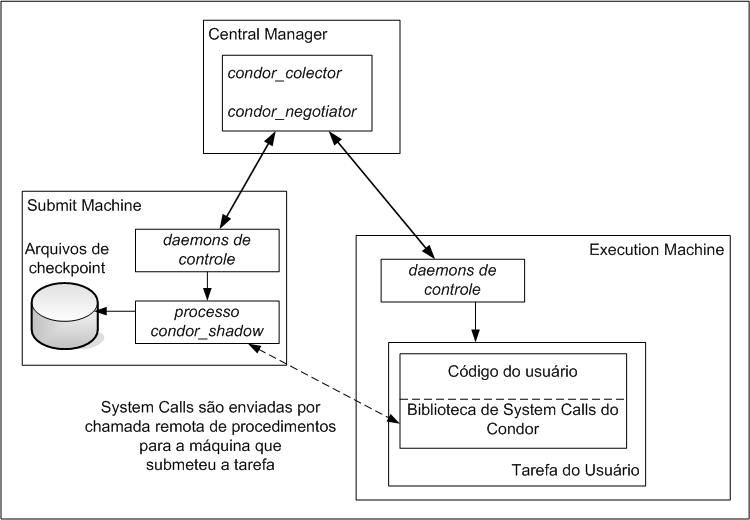
\includegraphics[width=10cm]{figures/condor.png}
  \caption[Arquitetura do Condor]{Arquitetura do Condor}
  \label{figure:condor1}
\end{center}
\end{figure}

Ainda na Figura~\ref{figure:condor1}, � mostrada a composi��o interna de cada componente. O Central Manager prov� dois servi�os b�sicos: (i) o \textit{condor\_collector}, que coleta informa��es dos componentes mantendo um hist�rico do estado da grade; e (ii) o \textit{condor\_negotiator}, respons�vel pelo \textit{matching} entre recursos dispon�veis e aplica��es submetidas. As \textit{Submit Machines} possuem v�rios daemons respons�vel pelo controle das tarefas em execu��o entre eles o \textit{condor\_shadow}, que atua como um gerente dos recursos para a aplica��o executando na \textit{Execution Machine}, isto �, ela recebe as \textit{system calls} da tarefa do cliente, executando no recurso doado (usando o ambiente de execu��o \textit{Standard}, explicado mais a frente) e redirecionadas pela API do Condor.

Num \textit{pool} Condor s� existe um �nico \textit{Central Manager}. Ele � respons�vel por coletar informa��es dos outros componentes e ainda por realizar o casamento entre recursos e tarefas. Caso essa m�quina falhe n�o ser� poss�vel mais executar nenhuma tarefa, apesar de que as tarefas j� em execu��o continuam a executar. Dada essa import�ncia, recomenda-se instalar o Central Manager numa m�quina com maior disponibilidade ou que possa ser reiniciada o mais r�pido poss�vel no caso de falha. Tamb�m se deve considerar recursos de disco e capacidade de tr�fego de rede para essa m�quina.

O \textit{middleware} est� dispon�vel para as plataformas Intel x86 e 64, PowerPC, SPARC e HP/PA, sendo poss�vel instalar em diferentes sistemas operacionais como MacOS, Linux Debian, Windows NT, Solaris, FreeBSD, AIX, HP/UX, RHEL, entre outros.

Existem \textit{pools} Condor espalhados por todo o mundo. Formar comunidades ou entrar numa comunidade formada depende das inten��es das entidade que mant�m cada uma delas. O administrador de um laborat�rio pode criar um pool com os recursos existentes e permitir a execu��o de tarefas de qualquer outro pool, por�m precisa de autoriza��o do administrador de um pool para usar seus recursos. Existem configura��es espec�ficas referentes � permiss�o de execu��o de aplica��es de outros pools e que precisam ser manualmente escolhidas. 

\subsubsection{XWHEP}

O XWHEP tamb�m possui tr�s componentes fundamentais (Figura~\ref{figure:xwhep1}): (i) o \textit{Server}, entidade centralizada encarregada de gerenciar a plataforma; (ii) o \textit{Worker}, software distribu�do nas m�quinas que ter�o seus recursos doados; e (iii) o \textit{Client}, software que interage com a plataforma submetendo tarefas.

\begin{figure}[htp]
\begin{center}
  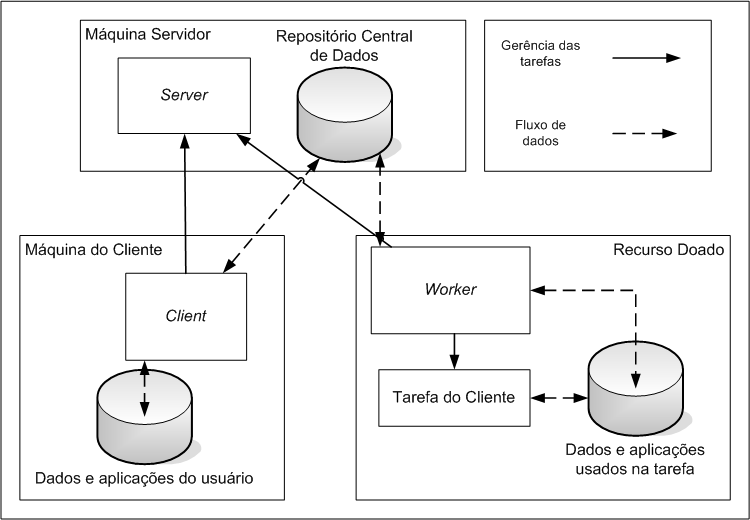
\includegraphics[width=10cm]{figures/xwhep.png}
  \caption[Arquitetura do XWHEP]{Arquitetura do XWHEP}
  \label{figure:xwhep1}
\end{center}
\end{figure}

Os componentes dependem fundamentalmente do \textit{Server} e n�o suportam falhas dele. O banco de dados central tamb�m � um ponto �nico de falha. 

O middleware � escrito na linguagem Java e portanto requer a JVM para compilar os pacotes. Por�m, a instala��o do server s� pode ser feita em m�quinas com Linux ou Mac OS X, enquanto Worker e Client podem ser instalados em em Linux, Windows (executando no ambiente Cygwin) e MacOS.
 
O XWHEP � usado pelo LAL~\cite{lal} para execu��o de aplica��es envolvendo f�sica de altas energias e usu�rios interessados em contribuir podem voluntariamente doar os ciclos ociosos de suas m�quinas, instalando o Worker, para a execu��o de aplica��es do LAL. No entanto n�o existe uma comunidade aberta onde o usu�rio possa tamb�m consumir recursos da grade.

\subsubsection{OurGrid}

O OurGrid possui quatro componentes fundamentais: (i) o \textit{Peer}, componente existente em cada site e respons�vel por fazer o casamento entre recursos e tarefas a serem executadas; (ii) o \textit{Discovery Service}, entidade centralizada encarregada de manter um cat�logo de \textit{Peers}; (ii) o \textit{Worker}, que executa nas m�quinas com recursos a serem doados; e (iii) o \textit{Broker}, que submete e acompanha a execu��o dos \textit{jobs} na grade. O \textit{Discovery Service} n�o acompanha a distribui��o padr�o oferecida na p�gina do OurGrid~\cite{ourgrid:site}. Um administrador que queira implantar uma comunidade a parte deve procurar uma vers�o est�vel no reposit�rio do c�digo ou entrando em contato com o time de desenvolvimento.

Na Figura~\ref{figure:ourgrid1}, � apresentada a distribui��o desses componentes em dois \textit{sites} distintos. Cada site representa um dom�nio administrativo diferente gerenciado por um \textit{peer}. Por ser um componente centralizado, o \textit{Discovery Service} � um ponto de falha. Entre suas atribui��es est�o a de manter a comunidade conectada, informando a cada \textit{Peer} a lista dos \textit{Peers} presentes na comunidade. Uma vez que este componente falhe, n�o ser� poss�vel a entrada de novos \textit{Peers} na comunidade. Atualmente, com a vers�o est�vel do \textit{Discovery Service}, � poss�vel instalar mais de um por comunidade, atuando como um servidor de replica��o.

\begin{figure}[htp]
\begin{center}
  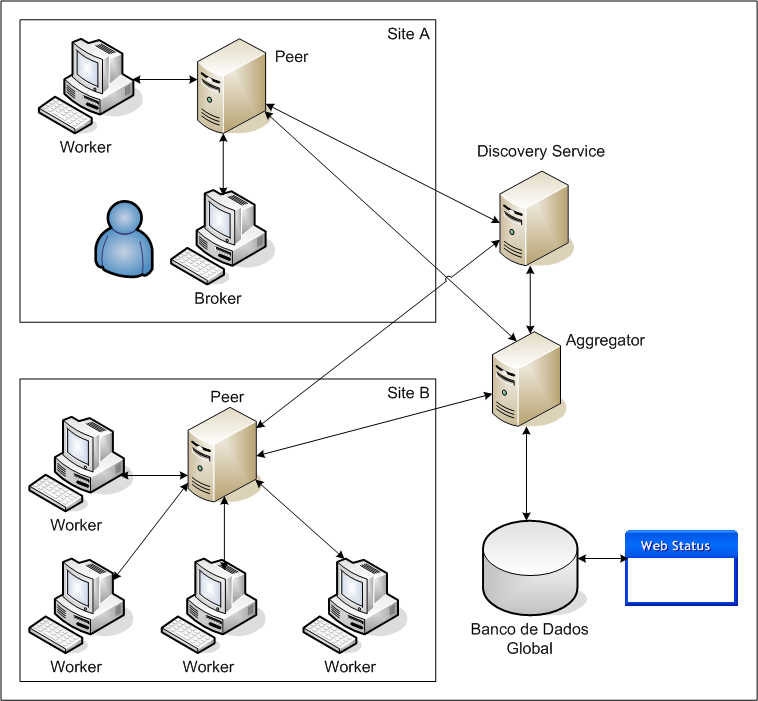
\includegraphics[width=10cm]{figures/og.png}
  \caption[Arquitetura do OurGrid]{Arquitetura do OurGrid}
  \label{figure:ourgrid1}
\end{center}
\end{figure}

Como o OurGrid � escrito na linguagem Java~\cite{java} e executa sobre a \textit{Java Virtual Machine} (JVM\nomenclature{JVM}{Java Virtual Machine}) � independente de plataforma e sistema operacional dado que estes d�em suporte a tecnologia Java.  

Atualmente, h� uma comunidade aberta \textit{free-to-join} do OurGrid liderada pelo LSD~\cite{lsd}. Qualquer interessado em usar o \textit{middleware} OurGrid pode ser juntar a comunidade compartilhando seus recursos.

\subsubsection{Configura��o}

O Condor segue o princ�pio de deixar todas as decis�es a crit�rio do usu�rio e isso o torna bastante dif�cil de configurar pois existem muitas decis�es a serem tomadas antes de iniciar a instala��o. As configura��es do Condor s�o divididas em quatro categorias: (i) obrigat�rias, sem elas a grade n�o funciona; (ii) obrigat�rias com op��es padr�o; (iii) pol�ticas de execu��o; e (iv) arquivos de log e op��es mais espec�ficas de cada tipo de aplica��o suportada.

� recomendado que os componentes do \textit{middleware} executem com privil�gio de super usu�rio dado que de outro modo qualquer pessoa poderia fazer com que os daemons do condor executassem programas maliciosos.

O Condor usa as portas 9618 e 9614 respectivamente para o coletor de dados e o negociador. Os outros servi�os executam usando portas escolhidas randomicamente pelo sistema mas que podem ser configuradas para usar a faixa padr�o de 9600 a 9700. O n�mero de portas no \textit{Central Manager} � determinado por informa��es como, por exemplo, o n�mero de m�quinas no pool, n�mero de processadores nos recursos doados e n�mero m�ximo de tarefas simult�neas nos recursos individualmente.   

Um caso similar � o XWHEP. A instala��o � bastante problem�tica dado que muitas das op��es de configura��o s�o obrigat�rias e confusas. Como a arquitetura da grade requer que todos os componentes tenham acesso a um �nico banco de dados usado para depositar os arquivos das aplica��es, � necess�rio que se proveja acesso ao banco a partir de todas as m�quinas na grade abrindo a porta 3306 usada pelo MySQL, o que nem sempre � uma pr�tica aceit�vel pelos administradores da rede. Al�m desta, outras portas precisam ser abertas para permitir comunica��o com o Server (4321 a 4329) e com o Worker (4323).

De todos os pacotes de \textit{middleware} analizados, o OurGrid � o que requer menos pa\-r�\-me\-tros de configura��o a serem atribu�dos. Como os componentes se comunicam atrav�s do protocolo Extensible Messaging and Presence Protocol (XMPP\nomenclature{XMPP}{Extensible Messaging and Presence Protocol}), � necess�rio que duas portas estejam abertas para comunica��o entre todos os componentes (por padr�o 5222 e 5223) e o servidor XMPP e uma porta no servidor aberta para comunica��o com o mundo (por padr�o, a porta 5269). A configura��o dos componentes � simples e pode ser feita usando a interface gr�fica ou por meio de comandos.

\subsection{Ger�ncia e Administra��o}

O Condor oferece alguns comandos pr�prios para administradores do sistema como o \textit{condor\_status} para buscar informa��es moment�neas da grade, como o estado das m�quinas que comp�em a grade ou as m�quinas dispon�veis para executar tarefas; e o \textit{condor\_stats} que prov� informa��es hist�ricas da grade armazenada no CentralManager. Exemplos das sa�das do comando \textit{condor\_status} podem ser encontradas na Figura~\ref{figure:code1} e~\ref{figure:code2}

\begin{figure}
\makebox[\textwidth]{\hrulefill}
\scriptsize
\begin{verbatim}
Name               JavaVendor Ver    State     Activity LoadAv Mem   ActvtyTime

slot1@ricardo0.lsd Sun Micros 1.6.0_ Owner     Idle     0.200   984  0+00:05:07
slot2@ricardo0.lsd Sun Micros 1.6.0_ Owner     Idle     0.000   984  0+00:05:08
slot1@ricardo1.lsd Sun Micros 1.6.0_ Owner     Idle     0.010   759  0+00:05:09
slot2@ricardo1.lsd Sun Micros 1.6.0_ Owner     Idle     0.000   759  0+00:05:10
slot1@ricardo2.lsd Sun Micros 1.6.0_ Unclaimed Idle     0.010   991  0+00:00:04
slot2@ricardo2.lsd Sun Micros 1.6.0_ Unclaimed Idle     0.000   991  0+00:05:06

                     Total Owner Claimed Unclaimed Matched Preempting Backfill

         INTEL/LINUX     6     4       0         2       0          0        0

               Total     6     4       0         2       0          0        0

\end{verbatim}
\makebox[\textwidth]{\hrulefill}
\caption{Sa�da do comando \textit{condor\_status}}
\label{figure:code1}
\end{figure}
\normalsize


\begin{figure}
\makebox[\textwidth]{\hrulefill}
\scriptsize
\begin{verbatim}
Name               OpSys      Arch   State     Activity LoadAv Mem   ActvtyTime

slot1@ricardo2.lsd LINUX      INTEL  Unclaimed Idle     0.010   991  0+00:00:04
slot2@ricardo2.lsd LINUX      INTEL  Unclaimed Idle     0.000   991  0+00:05:06

                     Total Owner Claimed Unclaimed Matched Preempting Backfill

         INTEL/LINUX     2     0       0         2       0          0        0

               Total     2     0       0         2       0          0        0
\end{verbatim}
\makebox[\textwidth]{\hrulefill}
\caption{Sa�da do comando \textit{condor\_status -available}}
\label{figure:code2}
\end{figure}
\normalsize

De modo similar o XWHEP oferece scripts para verificar o estado da grade. Tamb�m � poss�vel configurar par�metros dos Workers como, por exemplo, n�mero m�ximo de tarefas simult�neas e regras de ativa��o do Worker, via uma interface web fornecida pelo XWHEP~\ref{figure:xwworker}.

\begin{figure}[htp]
\begin{center}
  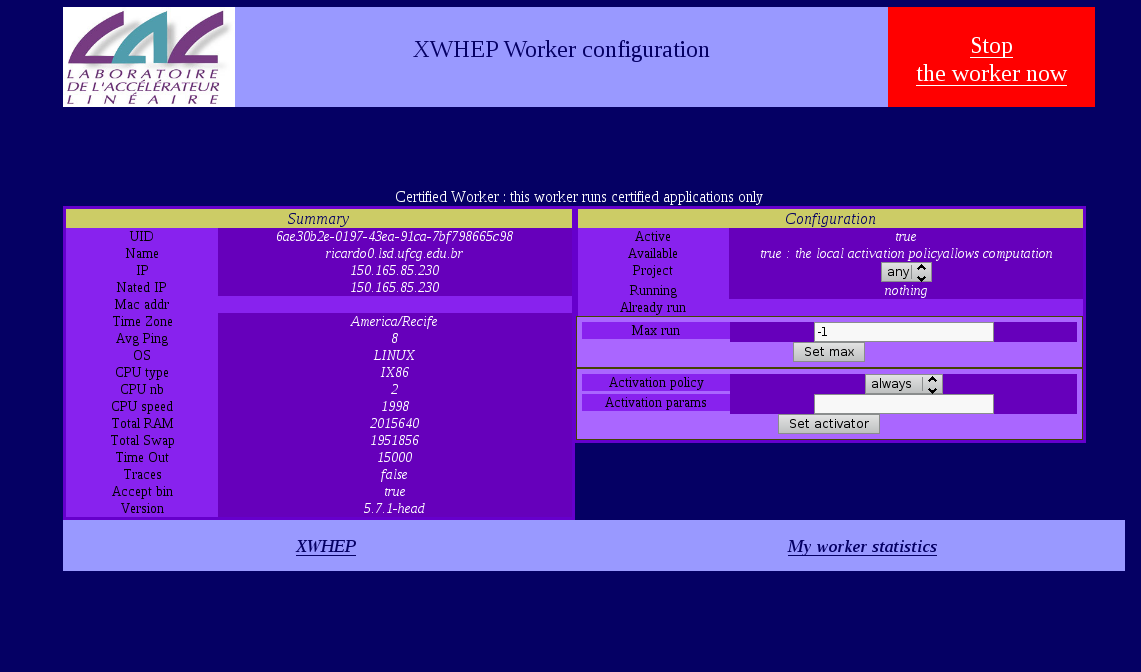
\includegraphics[width=15cm]{figures/xwworker.png}
  \caption[Configura��o do \textit{Worker} no XWHEP]{Configura��o do \textit{Worker} no XWHEP}
  \label{figure:xwworker}
\end{center}
\end{figure}
 
Por sua vez, o OurGrid disponibiliza o portal WebStatus com informa��es recentes sobre a grade como n�mero de Peers conectados, m�quinas dispon�veis e clientes executando tarefas no momento (ver Figura~\ref{figure:status}). Esses dados s�o coletados dos \textit{Peers} e \textit{Discovery Service} pelo \textit{Aggregator} periodicamente.

\begin{figure}[htp]
\begin{center}
  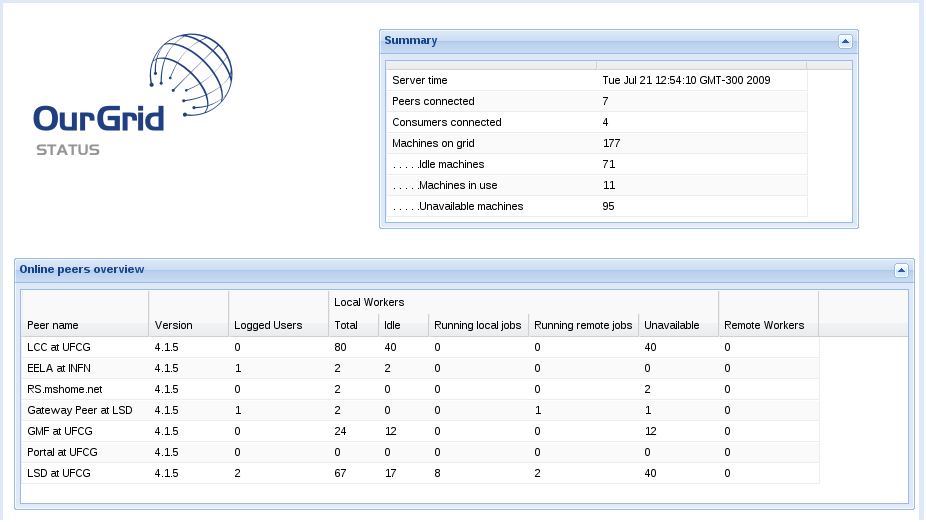
\includegraphics[width=15cm]{figures/status.png}
  \caption[OurGrid WebStatus]{OurGrid WebStatus}
  \label{figure:status}
\end{center}
\end{figure}

A pr�pria arquitetura do condor contribui para a prote��o do recurso doado diante de aplica��es maliciosas.  
O Condor permite a execu��o de VMs como se fossem aplica��es. A aplica��o � dada como finalizada quando a imagem � encerrada.

O XWHEP n�o suporta nenhum tipo de ambiente de execu��o virtualizado. J� o OurGrid Worker pode ser instalado numa m�quina virtual Vserver tendo os benef�cios deste tipo de ambiente de execu��o.

\subsection{Aplica��es}

No Condor os ambientes de execu��o s�o chamados de universos. Atualmente s�o disponibilizados nove universos, s�o eles:

\begin{itemize}
  \item \textit{Standard}: prov� \textit{checkpointing} e \textit{system calls} remotas, mas com restri��es;
  \item \textit{Vanilla}: sem \textit{checkpoint} e \textit{system calls} remotas. �til para programas que n�o podem ser ``relinkados'' e para scripts Shell. Os arquivos de entrada e sa�da podem estar num sistema de arquivos compartilhados ou pode ser usada o mecanismo de transfer�ncia de arquivos do Condor;
  \item \textit{Grid}: permite ao usu�rio submeter tarefas para sistemas com interface similar ao Globus Toolkit usando o Condor;
  \item Java: Tarefas BoT escritas para a JVM;
  \item \textit{Scheduler}: permite submeter tarefas leves para o daemon \textit{condor\_schedd} (futuramente substitu�do pelo universo Local);
  \item \textit{Local}: Executa logo que submetido na m�quina local sem esperar por \textit{matching} com outra m�quina (a tarefa iniciada n�o pode ser mais preemptada);
  \item \textit{Parallel}: para programas que necessitam de v�rias m�quinas por tarefa como, por exemplo, as escritas usando o padr�o MPI;
  \item VM: usado quando a tarefa n�o � s� uma aplica��o, mas uma imagem de disco (facilita a execu��o de m�quinas virtuais) VMware ou Xen.
\end{itemize}

Uma vez escolhido um universo adequando a aplica��o que se deseja executar, � necess�rio escrever um \textit{Submit Description File} (SDF) no qual ser� indicado o universo escolhido, os arquivos da aplica��o, o modo de transfer�ncia entre outras informa��es. Um exemplo de SDF � mostrado em \ref{figure:code3}. Uma aplica��o Java � posta na fila de execu��es. O Java Archive (JAR) da aplica��o � submetido e a classe \texttt{sim.core.Preprocess} � executada tendo como arquivo de entrada ``raw\_data.dat'' localizado na m�quina que submete a tarefa, a partir da pasta corrente, no caminho ``simulator/input/'', e cujos arquivos de sa�da sim\_output e sim\_error ser�o transferidos ao final da execu��o.

\begin{figure}
\makebox[\textwidth]{\hrulefill}
\scriptsize
\begin{verbatim}
universe = java
executable = sim.jar
jar_files = sim.jar
arguments = sim.core.PreProcess raw_data.dat
transfer_input_files = simulator/input/raw_data.dat
output = sim_output
error = sim_err
should_transfer_files = YES
when_to_transfer_output = ON_EXIT
queue
\end{verbatim}
\makebox[\textwidth]{\hrulefill}
\caption{Condor Submit Description File}
\label{figure:code3}
\end{figure}
\normalsize

O Condor ainda permite que tarefas sejam executadas respeitando um Grafo Ac�clico Direcionado (Directed Acyclic Graph ou DAG\nomenclature{DAG}{Directed Acyclic Graph}). Isso � �til quando uma tarefa depende dos resultados de outras.

O XWHEP executa aplica��es Java e arquivos execut�veis nos sistemas operacionais suportados (Linux, Mac OS X e Windows). Tanto o arquivo da aplica��o como os dados de entrada s�o tratados como dados puros e para executar um comando � necess�rio deix�-los acess�veis via um Identificador de Recursos Uniforme (\textit{Unified Resource Identifier} ou URI\nomenclature{URI}{Unified Resource Idintifier}).

O OurGrid suporta, de maneira similar, aplica��es Java e arquivos execut�veis nos sistemas operacionais suportados. Por�m os arquivos da aplica��o ficam na m�quina onde est� o Broker. Uma vez que um novo Worker seja escolhido para executar a tarefa, os arquivos s�o transferidos e a tarefa inicia s� ap�s completar esta transfer�ncia. As aplica��es s�o submetidas por meio de um arquivo de metadados chamado Job Descriptor File (JDF\nomenclature{JDF}{Job Descriptor File}). O exemplo de JDF na Figura~\ref{figure:code4} � referente � execu��o da classe ``StartSim'' contida no jar ``sim.jar'' e tendo como entrada alguns argumentos num�ricos e o arquivo de entrada sim.dat.

\begin{figure}
\makebox[\textwidth]{\hrulefill}
\scriptsize
\begin{verbatim} 
job : 
label   : Job1

task :
init    : put sim.jar sim.jar
			store sim.dat sim.dat
remote  : java -cp sim.jar. StartSim 1000 864000 sim.dat output-$JOB.$TASK
final   : get output-$JOB.$TASK output-$JOB.$TASK
\end{verbatim}
\makebox[\textwidth]{\hrulefill}
\caption{OurGrid Job Description File}
\label{figure:code4}
\end{figure}
\normalsize


\subsection{Usando a grade}

\subsubsection{Detec��o de Ociosidade}

Nesse tipo de grade computacional aplica��es do usu�rio do recurso devem ser priorizadas em rela��o �s executadas na grade. para isso s�o necess�rios mecanismos que detectem e informem � grade sobre a disponibilidade do recurso. No Condor a ociosidade � regulada atrav�s de uma express�o no arquivo de configura��o do recurso. Essa express�o, chamada \textit{ClassAd} (\textit{classified advertisement}) tamb�m � enviada ao \textit{Central Manager} para ser usada na etapa de \textit{matching} entre as aplica��es submetidas a grade e os recursos dispon�veis. Um exemplo de ClassAd � dado na Figura~\ref{figure:classad} em que um recuso estar� dispon�vel na grade assim que a m�dia de carga for menor que 30\% e o teclado esteja inativo a mais de quinze minutos.

\begin{figure}
\makebox[\textwidth]{\hrulefill}
\scriptsize
\begin{verbatim}
[
MyType="Machine"
TargetType="Job"
Machine="machine1.lsd.ufcg.edu.br"
Requirements=(LoadAvg <= 0.3) \&\& (KeyBoardIdle > (15 * 60))
]
\end{verbatim}
\makebox[\textwidth]{\hrulefill}
\caption{ClassAd do Condor}
\label{figure:classad}
\end{figure}
\normalsize

A ativa��o do Worker no XWHEP tamb�m � determinada por um par�metro no arquivo de propriedades. As op��es dispon�veis s�o:

\begin{description}
  \item[\textit{AlwaysActive}:] � a op��o padr�o, na qual o worker est� apto a executar tarefas;
  \item[\textit{DateActivator}:] A disponibilidade � monitorada por data e tempo com sintaxe similar a do \textit{crontab};
  \item[\textit{CpuActivator}:] Disponibilidade regulada pela carga da CPU e dispon�vel somente para \textit{Workers} em Linux;
  \item[\textit{MouseKdbActivator}:] O Worker est� dispon�evl 30 segundos ap�s o dono ter usado o mouse ou teclado pela �mtima vez. N�o funciona para Mac OS X;
  \item[\textit{WinSaverActivator}:] Assim que a prote��o de tela for ativada o Worker entra em modo dispon�vel.   
\end{description}

OurGrid Worker � feita automaticamente, e de maneira similar ao \textit{MouseKdbActivator} do XWHEP, pelo monitoramento da atividade do mouse e teclado.

\subsubsection{Mecanismos de Incentivo}

Para incentivar a doa��o de recursos, o OurGrid implementa a Rede de Favores (\textit{Network of Favors} ou NoF\nomenclature{NoF}{Network of Favors}). A NoF intentiva intera��es com Peers colaboradores e desincentiva \textit{free-riders}, que s�o peers que s� consomem recursos. Esse incentivo � realizado com base em intera��es passadas mantidas no hist�rico de cada \textit{Peer}. No Condor � poss�vel priorizar aplica��es usando ass express�es ClassAds na configura��o da m�quina. Por exemplo, adicionando a linha \verb!Rank = Owner == ``ricardo''! a m�quina configurada com o ClassAd na Figura~\ref{figure:classad} prioriza aplica��es submetidas por pelo cliente do usu�rio ricardo. Por fim, n�o existem mecanismos similares no XWHEP.


\subsubsection{Checkpoint}

Dada a volatilidade dos recursos, caracter�stica inerente �s grades computacionais de \textit{desktops}, as tarefas podem ser interrompidas e o trabalho computado perdido. O mecanismo de chackpoint permite arquivar o estado atual de execu��o de uma tarefa preemptada para uma posterior execu��o no mesmo recurso ou em um recurso diferente atrav�s da migra��o dessas informa��es. O condor, diferentemente do XWHEP e do OurGrid, permite fazer checkpoint no universo \textit{Standard}. No entando algumas restri��es s�o impostas entre elas:

\begin{itemize}
  \item � necess�rio ``relinkar'' a aplica��o usando o \textit{condor\_compile};
  \item N�o � permitido a cria��o de m�ltiplos processos;
  \item S� � permitida uma \textit{thread} no n�vel do \textit{kernel};
  \item N�o � permitido mapear arquivos na mem�ria (chamadas chamadas \textit{mmap()} e \textit{munmap()});
  \item S� permite manipula��o de arquivos menores que 2 GB.
\end{itemize}  

\section{Resultados Obtidos}

Como resultado da avalia��o foi constru�da a Tabela~\ref{table:resultados}.

\begin{center}
\footnotesize
\begin{longtable}{|p{4cm}|p{3cm}|p{3cm}|p{3cm}|} \hline

\hline \multicolumn{1}{|p{4cm}|}{\textbf{M�trica Observada}} & \multicolumn{1}{p{3cm}|}{\textbf{Condor}} & \multicolumn{1}{p{3cm}|}{\textbf{XWHEP}} & \multicolumn{1}{p{3cm}|}{\textbf{OurGrid}} \\ \hline 
\endfirsthead

\multicolumn{4}{c}%
{{\bfseries \tablename\ \thetable{} -- continua��o da p�gina anterior}} \\
\hline \multicolumn{1}{|p{4cm}|}{\textbf{M�trica Observada}} &
\multicolumn{1}{p{3cm}|}{\textbf{Condor}} &
\multicolumn{1}{p{3cm}|}{\textbf{XWHEP}} &
\multicolumn{1}{p{3cm}|}{\textbf{OurGrid}} \\ \hline 
\endhead

\hline \multicolumn{4}{|r|}{{Continua na pr�xima p�gina}} \\ \hline
\endfoot

\endlastfoot

Componentes Principais & 3 & 3 & 3 \\ \hline
Sistemas Operacionais suportados & Linux Debian, Windows NT, MacOS & Linux, Windows (Cygwin) e MacOS & Qualquer sistema operacional com suporte a Java\\ \hline
Configura��o & Muitas propriedades precisam ser especificadas para p�r a grade em funcionamento & Poucas propriedades s�o necess�rias, mas requer um banco de dados central configurado & Poucas propriedades s�o obrigat�rias \\ \hline
Executa em modo ``super-usu�rio'' & Sim & Sim & N�o \\ \hline
Portas abertas no Firewall & 2 no \textit{Central Manager} + faixa din�mica (por padr�o 100) & 9 & 3 \\ \hline
Necessita de negocia��o para entrar numa grade existente? & Administrador do pool deve configurar & N�o existe uma grade aberta & N�o \\ \hline
Existem ferramentas de gerencia? & Sim & Sim & Sim \\ \hline 
Suporte ao uso de tecnologia de virtualiza��o? & Sim & N�o & Sim\\ \hline 
� oferecido algum tipo de prote��o da m�quina doada? & Execu��o em \textit{sandbox} & N�o & Pode ser executado com Vserver\\ \hline 
Tipos de aplica��es suportados & BoT, MPI, Paralelas acopladas & BoT, MPI & BoT\\ \hline
� neces�rio modificar as aplica��es? & Sim\footnote{No caso do uso de checkpoint}/N�o & N�o & N�o\\ \hline
Mecanismos de detec��o de ociosidade & Sim & Sim & Sim \\ \hline
Mecanismos de incentivo & N�o & N�o & Sim\\ \hline
Mecanismo de checkpoint & Sim & N�o & N�o\\ \hline
Comunidade ativa & Usu�rio pode doar recursos & Usu�rio pode doar recursos & Usu�rio pode doar e usar recursos\\ \hline
\caption[Resultados da avalia��o]{Resultados da avalia��o}
\label{table:resultados}
\end{longtable}
\end{center}

Os resultados apresentados nessa tabela s�o �teis para a tomada de decis�o sobre qual pacote de \textit{middleware} escolher para instalar num ambiente com computadores \textit{desktop} dispon�veis e que haja demanda por executar aplica��es que n�o sejam poss�veis, por quest�es de tempo ou demanda, de ser executadas usando a infraestrutura local.

Diferentes situa��es podem ser consideradas ao tomar esse tipo de escolha. No caso em que a urg�ncia em p�r a grade computacional em funcionamento � um fator determinante, pacotes de middleware cuja instala��o e configura��o exigem menos conhecimento acerca da grade s�o preferencialmente escolhidos. Esse � o caso do OurGrid.

Por outro lado, quando uma flexibilidade maior � requerida em termos de configura��es e tipos de aplica��es a serem executadas, caso em que o perfil dos usu�rios varie bastante, um pacote de \textit{middleware} mais flex�vel como o Condor � mais recomendado.

Esses resultados apresentados necessitam de um maior rigor metodol�gico, no entanto, servem como guia para administradores e usu�rios que desejam melhor utilizar seus recursos   

\chapter{Considera��o Finais}
\label{consideracoes}

%Descrever sobre a import�ncia do est�gio realizado para a sua forma��o, as dificuldades encontradas na realiza��o do est�gio (destacar aspectos positivos e negativos) e finalizar com coment�rios, apresentando sugest�es se achar necess�rio.

O est�gio trouxe novos conhecimentos a forma��o do estagi�rio como bacharelando em Ci�ncia da Computa��o assim como deu oportunidade de p�r em pr�tica alguns t�picos abordados em disciplinas te�ricas. T�picos muito importantes foram os relacionados � Ger�ncia e Configura��o de Redes de Computadores, os quais s�o oferecidos em disciplinas optativas. T�picos te�ricos das disciplinas Sistemas Operacionais, do curr�culo obrigat�rio, e Sistemas Distribu�dos, do curr�culo optativo, foram de fundamental import�ncia desde a etapa de levantamento bibliogr�fico como tamb�m configura��o do ambiente. Grande parte da teoria vista nas disciplinas contribuiu de certo modo para a montagem do trabalho final. 

Foi sentida uma dificuldade em se organizar e por em pr�tica esse tipo de pesquisa com objetivos voltados a obten��o de resultados qualitativos. A disciplina de Metodologia Cient�fica poderia ser adaptada para explorar esse tipo de pesquisa que apesar de pouco comum na �rea de ci�ncias exatas pode fundamentar um trabalho mais qualitativo com os seus resultados.

Quanto ao trabalho realizado, alguns pontos negativos podem ser citados como: a op��o por usar aplica��es com alta demanda de CPU e pouca de dados teve como objetivo simplificar a an�lise realizada. Avaliar aplica��es \textit{data intensive} requer uma metodologia mais quantitativa para avaliar a efic�cia dos mecanismos empregados. No entanto, a pesquisa feita permitiu construir a classifica��o dos middlewares mesmo sem usar tais tipos de aplica��es dado que as caracter�sticas avaliadas puderam ser extra�das mesmo sem o uso de uma metodologia mais apurada quantitativamente.

O trabalho realizado pode ser estendido para incluir aplica��es paralelas fortemente acopladas (em que as tarefas se comunicam, a exemplo de MPI) visto que algumas das grades d�o suporte � execu��o desse tipo de aplica��o. Um trabalho similar pode ser realizado considerando grades de servi�o tais como Globus ou at� comparando o estado da pr�tica entre as grades de servi�o com as grades de Desktop oportunistas.

Observou-se que o OurGrid � o �nico que possui uma grade existente que � \textit{free-to-join} e \textit{free-to-execute}, isto �, aberta para a doa��o de recursos e uso de recursos para aplica��es do usu�rio. No entanto, o OurGrid d� suporte apenas � execu��o de aplica��es BoT, o que nem sempre satisfaz todos os usu�rios.

O Condor mostra-se o \textit{middleware} mais est�vel e que det�m a maior comunidade (quando se considera a uni�o de v�rios pools). Por ter como objetivo a flexibilidade, aceita di\-fe\-ren\-tes tipos de aplica��es com diferentes requisitos, por�m �s custas de uma configura��o cara.

Por fim, o XWHEP possui uma organiza��o diferente em que os dados s�o disponibilizados por URIs e existe controle de acesso. Dessa forma as aplica��es maliciosas n�o podem apagar dados do servidor. No entanto, a exist�ncia de um banco de dados central do qual todos os componentes dependem � uma preocupa��o para administradores da grade computacional.


\bibliographystyle{plain}
\bibliography{relatorio}

\appendix

\chapter{Plano de Est�gio}

\end{document}
